% Asset ID: AS1TrigonometricRatiosTIKZ-002
% Source: P1-Chp9 pp.7-8
% Related section: Cosine Rule
% Purpose: Cosine rule triangle labelling
\documentclass[tikz,border=8pt]{standalone}
\usepackage{amsmath}
\usetikzlibrary{angles,quotes,calc,arrows.meta}
\begin{document}
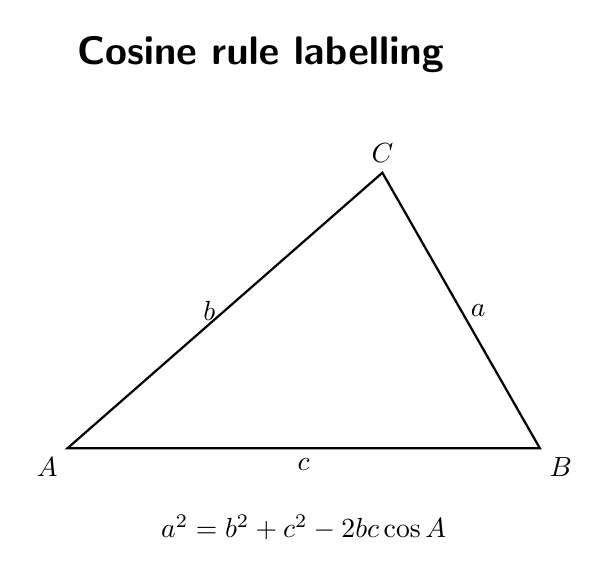
\begin{tikzpicture}[scale=1.0, every node/.style={font=\sffamily}]
\node[font=\sffamily\bfseries\Large, anchor=west] at (0,5) {Cosine rule labelling};
\coordinate (A) at (0,0);\coordinate (B) at (6,0);\coordinate (C) at (4,3.5);\draw[thick] (A)--(B)--(C)--cycle;\node[below left] at (A) {$A$};\node[below right] at (B) {$B$};\node[above] at (C) {$C$};\node[right] at ($(B)!0.5!(C)$) {$a$};\node[left] at ($(A)!0.5!(C)$) {$b$};\node[below] at ($(A)!0.5!(B)$) {$c$};\node at (3,-1) {$a^2=b^2+c^2-2bc\cos A$};
\end{tikzpicture}
\end{document}
